\chapter{Проверка работы устройства}
\label{cha:pract}

\section{Ping-Pong}

Было собрано два идентичных устройства и портирован код приложения Ping-Pong, 
являющийся в беспроводных приложениях подобием доказательства концепции 
(\textit{proof of concept}).

Приложение было модернизировано, добавление системы логирования и счётчиками 
отправленных и принятых пакетов.
Логирование осуществлялась посредством виртуального COM интерфейса STM32L4.
Во время подключения к компьютеру плата отправляет через COM интерфейс 
отладочные данные. 
Пример отладочных данных дан ниже:
\textfile[firstline=6,lastline=11]{inc/src/N61.76196E34.36578.txt}

Полный исходный код приложения Ping-Pong будет дан в приложении 
\ref{cha:appendix1}.

\section{Проверка работы приёмопередатчиков}

Для проверки работы приложения и оценки качества сигнала одно из устройств было 
оставлено на высоте 18 метров (5 этаж дома) с автономным источником питания 
(см. рис. \ref{fig:exp1}.
Второе устройство было взято с собой для измерения сигнала. 
В результате была установлена связь с между модулями и оценено качество связи 
по параметру Packet Error Rate (\textbf{PER}). 
Это отношение пропущенных (не принятых) пакетов к общему количеству 
отправленных.

\begin{figure}[!h]
  \centering
  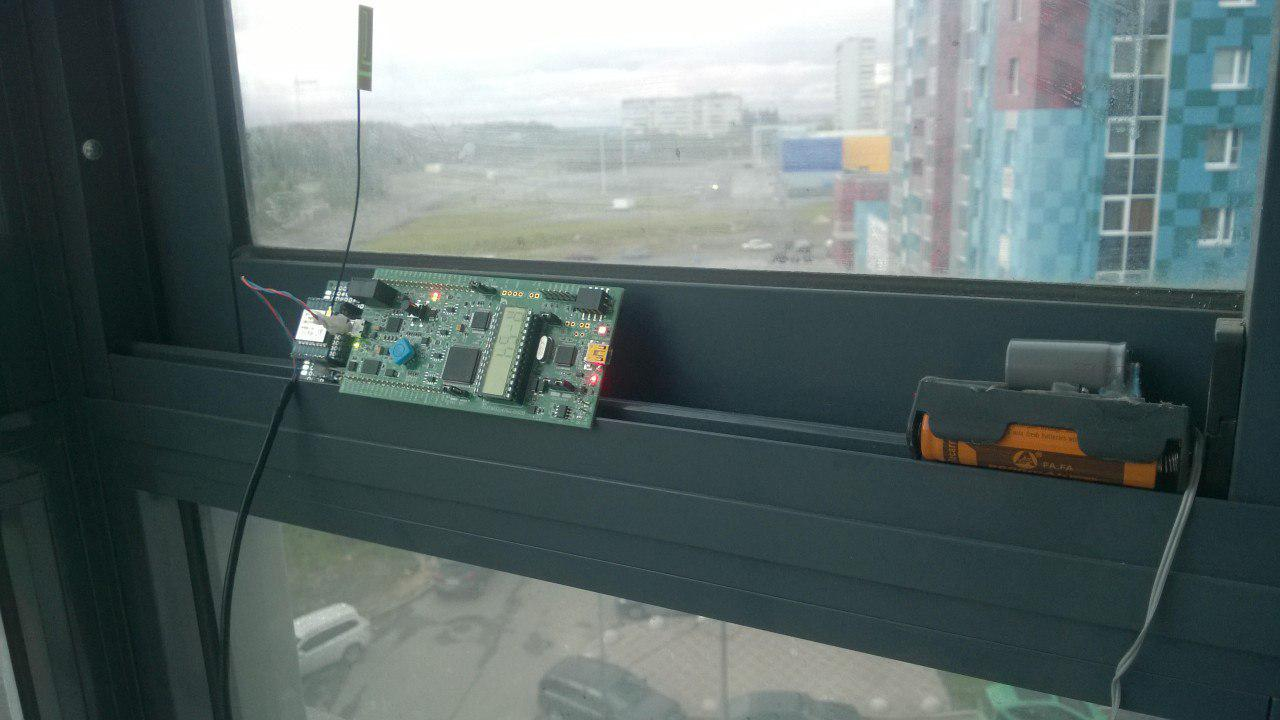
\includegraphics[width=\textwidth]{inc/img/exp1}
  \caption{Автономное устройство передающее кадры с Ping в приложении Ping-Pong}
  \label{fig:exp1}
\end{figure}

Результаты измерений отображены на рисунке \ref{fig:measmap} и в таблице 
\ref{tab:meastab}.

\begin{table}[ht]
  \caption{Результаты замеров}
  \begin{tabular}{|l|c|c|c|}
\hline
\begin{tabular}[c]{@{}l@{}}Описание \\ места\end{tabular}                        
                & \begin{tabular}[c]{@{}c@{}}Расстояние \\ до БС, м\end{tabular} 
& PER, \%      & RSSI                                                  \\ \hline
\begin{tabular}[c]{@{}l@{}}За домом.\\ Несколько стен.\end{tabular}              
                & 40                                                             
& 0,8 & -94                                                   \\ \hline
\begin{tabular}[c]{@{}l@{}}Улица.\\ Прямая видимость БС\end{tabular}          
                & 293                                                            
& 1            & -88                                                   \\ \hline
\begin{tabular}[c]{@{}l@{}}В магазине\\ Видимости нет.\\ Глубоко 
внутри помещения\end{tabular} & 280                                              
              & 100          & \begin{tabular}[c]{@{}c@{}}Нет\\ 
сигнала\end{tabular} \\ \hline
\begin{tabular}[c]{@{}l@{}}Улица.\\ Прямой\\ видимости нет.\\ Рельеф 
закрывает БС\end{tabular} & 687                                                  
          & 14,9         & -102                                                 
 \\ \hline
\begin{tabular}[c]{@{}l@{}}Улица. Прямой \\ видимости нет. \\ Плотная 
застройка.\end{tabular}    & 524                                                 
           & 24,4         & -112                                                 
 \\ \hline
\end{tabular}
  \label{tab:meastab}
\end{table}

Используемые параметры физического уровня: модуляция LoRa, SF = 7, BW = 125 
кГц, несущая частота равна 433 МГц, CR = 4/5, длина преамбулы равна 8, усиление 
передатчика - 14 дБ.

\begin{figure}[!h]
  \centering
  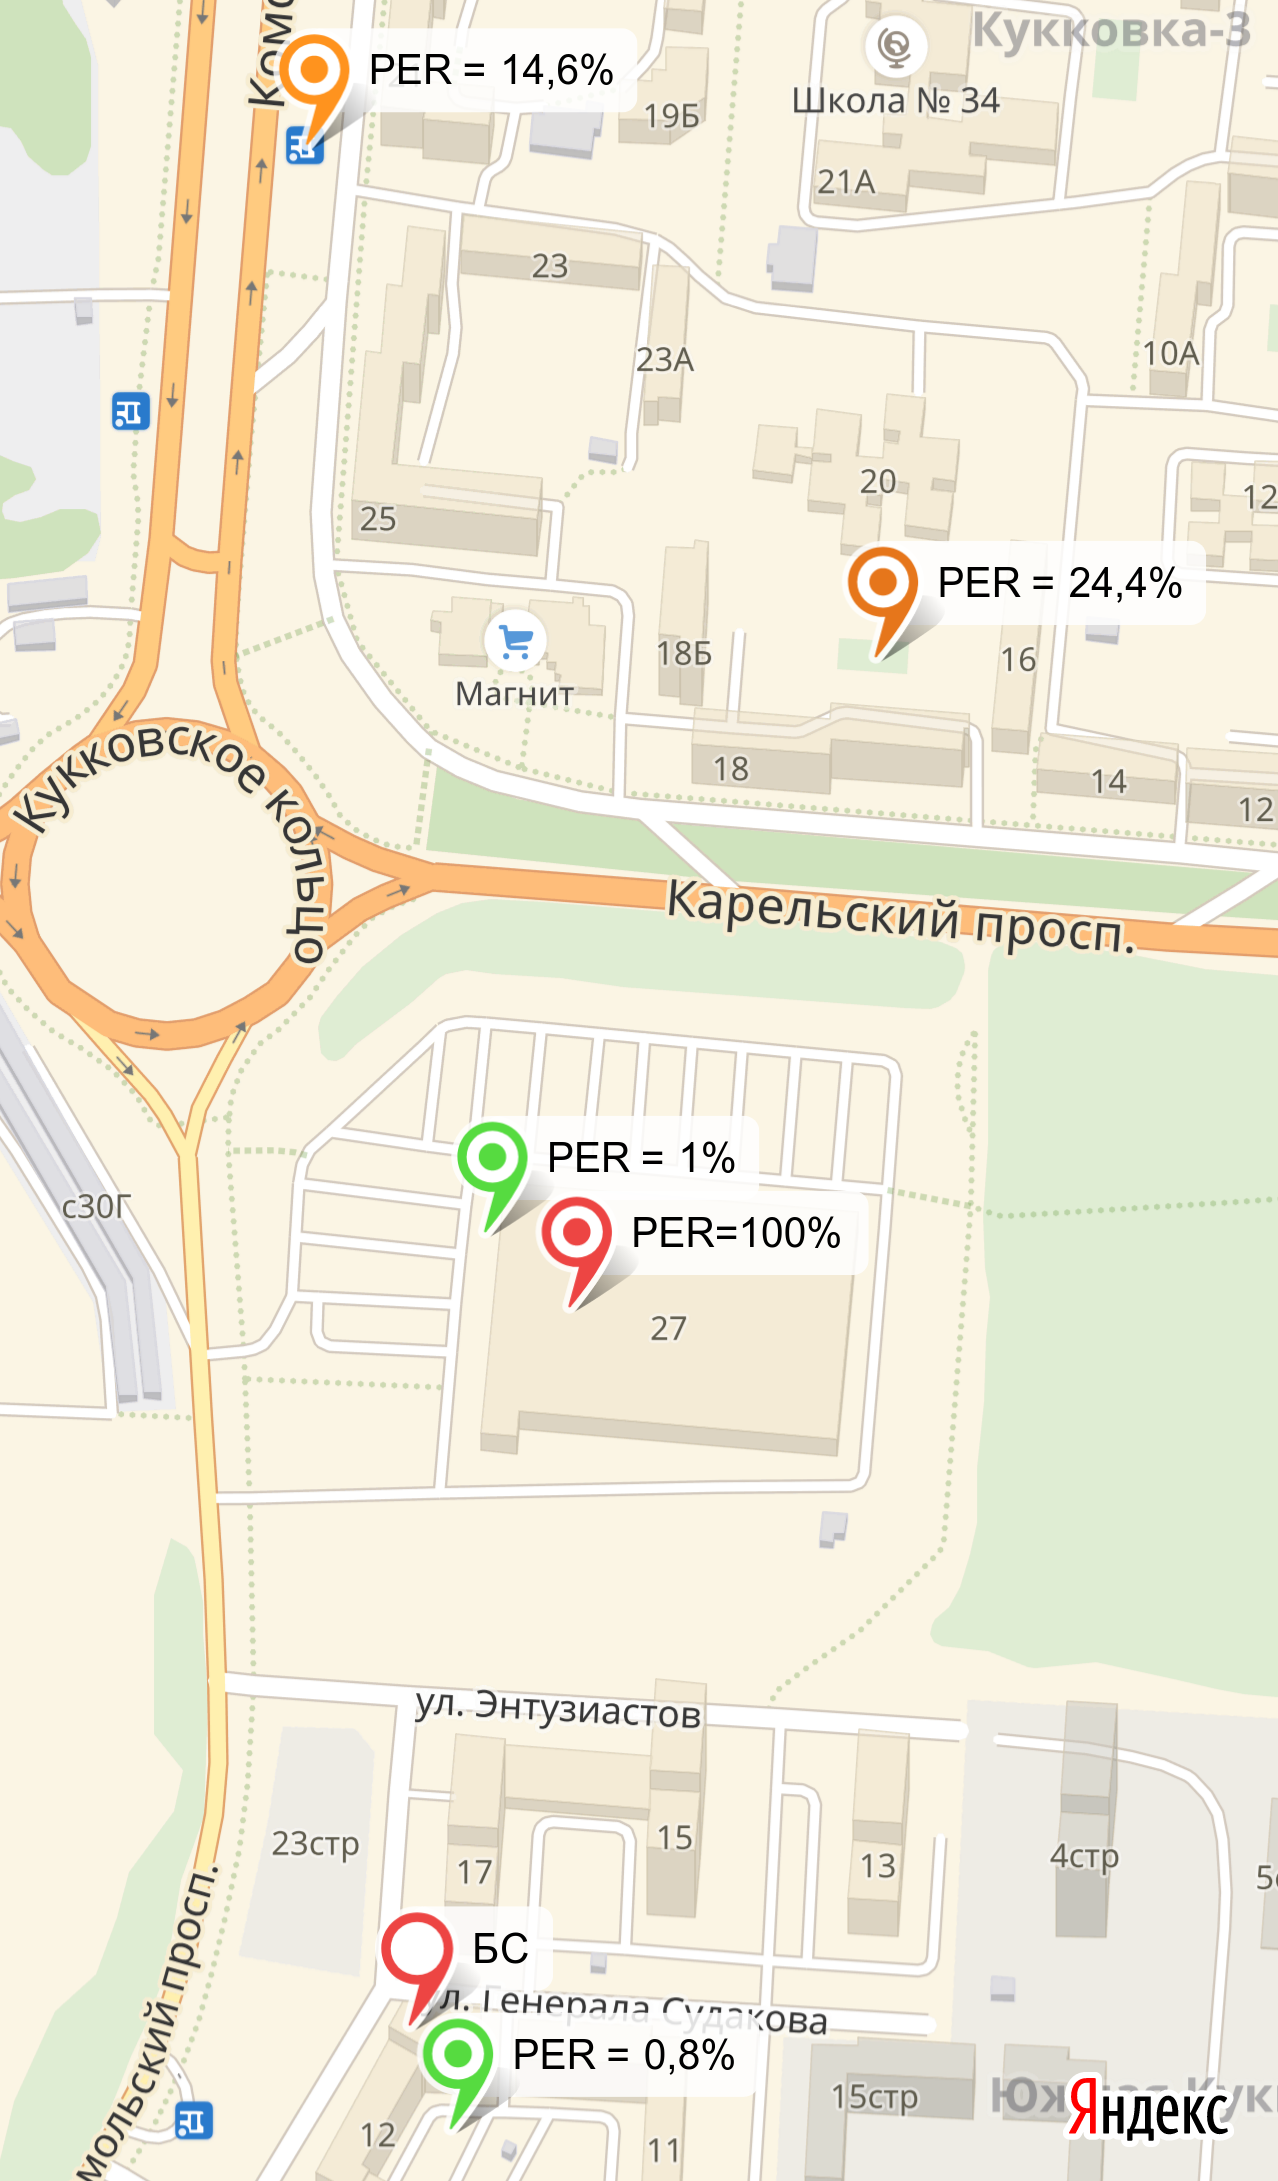
\includegraphics[height=\textheight]{inc/img/LoRaMeas}
  \caption{Результаты замеров качества приёма пакетов}
  \label{fig:measmap}
\end{figure}